El enunciado presenta el problema de hallar el camino entre 2 puntos que se pueda recorrer en el menor tiempo posible, dandonos un escenario en donde los caminos presentan paredes que podemos atravezar rompiendolas, teniendo a la vez, una determinada cantidad de rupturas a poder realizar. La solución buscada será entre todos los caminos posibles desde el origen al destino, el que resulte mínimo.

Cada camino esta compuesto de unas unidades "caminables", que las llamaremos baldozas. Ir de una baldoza a otra consume la misma cantidad de tiempo en todos los casos. Por otro lado, hay 
baldozas que demandan romper una pared para ser caminadas, con lo cual el camino que se esta transitando debe gastar 1 unidad de esfuerzo en romperla, factor que no influye en el tiempo del recorrido.

Si caracterizamos cada baldoza con un nodo, y la posibilidad de ir de una baldoza a otra como una arista, entonces podemos modelar el problema con un grafo. Como el factor tiempo es constante en cada traslado entre baldozas, las aristas tendrán todas el mismo peso.

A partir de este grafo, sacar el camino mínimo del nodo origen al destino se puede realizar utilizando el algoritmo de busqueda por anchura, el cual permite saber la distancia (o tiempo) a la que se encuentra determinado nodo con cada uno de los demas. Para ello el BFS utiliza una cola donde introduce nodos que aún no fueron marcados como visitados, para luego extraerlos de a uno y encolar las repectivas adyacencias que aún no fueron visitadas. Cada nodo pusheado a la cola representa, de esta manera, la cabeza de cada camino que forma el BFS para formar el árbol. 

Como no hay ninguna otra restricci\'on para encolar un nodo (y as\'i descubrir un camino), de aplicar el BFS sin modificaciones se perdería la restricci\'on de paredes para romper: por esto se debe agregar una validación al introducir un nodo a la cola del algoritmo, que impida pushear un nodo que demande romper más paredes de las parametrizadas.

Dado que al marcar un nodo como visitado se lo esta excluyendo de ser incluido en la cola nuevamente, de haber otro camino que lo necesite utilizar, el mismo no podrá contar con él. De suceder, se podr\'ia estar desestimando caminos que lleguen a la soluci\'on: Si llamamos $C_0$ al primer camino que paso por el nodo $v_0$ con tiempo 5 y paredes rotas 4, siendo el m\'aximo 4 y $C_1$ a un camino más lento, con tiempo 10 pero con 0 paredes rotas, que está pasando por $v_0$, entonces en la evaluación de agregar o no al nodo se optará por no, ya que fue visitado. No obstante, si para llegar al destino final se debe romper 1 pared más, $C_0$ nunca podrá llegar, y $C_1$ que hubiese llegado, fue desestimado anteiormente, perdiendo de esta forma la solución factible.

Para solucionar este problema se redefine la condición de visitado que utiliza el BFS:

  \vspace*{0.3cm} \vspace*{0.3cm}
  \begin{center}
 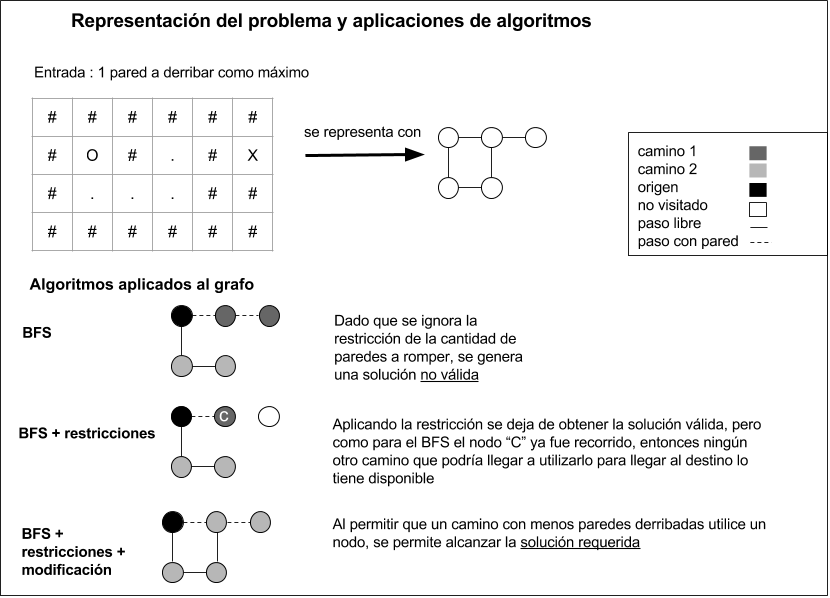
\includegraphics[scale=0.6]{./EJ1/ej1-explicacion.png}
  \end{center}
  \vspace*{0.3cm}

Se considerará que la condición de visitado dependa de cada camino, es decir:

\begin{itemize}
	\item Los nodos guardarán como datos propios el tiempo en el que fueron alcanzados y la cantidad de paredes que fueron destruidas para llegar a él en ese tiempo (es decir, los datos del camino que paso por él). Al inicio, ambos par\'ametros serán marcados como no determinados.
	\item Al ser chequeados por primera vez, al detectarse de que no tienen datos, entonces se les asignará el tiempo en el que fueron alcanzados (como en el algoritmo BFS original) y la cantidad de paredes derribadas para alcanzarlos.
	\item Si al chequearlos nuevamente se ve que ya fueron recorridos (es decir que el tiempo y paredes se encuentran determinados) entonces se evaluará si por el camino actual {\bf se mejora la condición del alcance del nodo} , de ser asi, se encola.
	\item En todos los casos, si al chequear un nodo, se detecta que hay que romper una pared, y el camino actual no posee más derribos posibles, entonces no se lo pushea a la cola.
	\item Si el nodo es el destino buscado, se lo marca con el tiempo y paredes logradas y se {\bf finaliza el algoritmo}.
	
\end{itemize}

\subsubsection*{Condición de alcance del nodo}
Se considera una mejor condición de alcance para un nodo si se cumple lo siguiente:
\begin{itemize}
	\item El nodo no tiene datos determinados, es decir nunca fue pusheado a la cola.
	\item La cantidad de paredes para llegar a él es menor estricta que la lograda anteriormente para llegar al nodo.

\end{itemize}